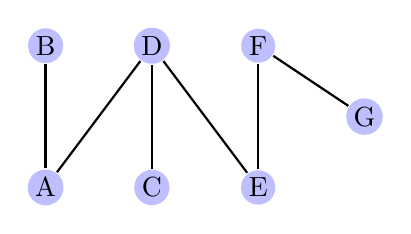
\begin{tikzpicture}[thick,scale=.45,auto=left,every node/.style={circle,fill=blue!25},inner sep=1pt,minimum size=2pt]
		  \node (n6) at (3,2) {A};
		  \node (n4) at (3,6) {B};
		  \node (n5) at (6,2) {C};
		  \node (n1) at (6,6) {D};
		  \node (n2) at (9,2) {E};
		  \node (n3) at (9,6) {F};
		  \node (n7) at (12,4) {G};
		  \foreach \from/\to in {n6/n4,n6/n1,n1/n5,n1/n2,n2/n3,n3/n7}
		    \draw (\from) -- (\to);
		\end{tikzpicture}